\subsection{\label{sec:radio}The Radio Lightcurve}
Radio Observations took place on April 8th, 2024 at the University of Central Arkansas campus in Conway, Arkansas at approximately 35$^\circ$04'51"N 92$^\circ$27'36"W with an elevation of 94 m.
We began collecting data at 2460409.2186657293 JD and ended at 2460409.3424835186 JD, or 2024-04-08 17:14:53 UTC and 2024-04-08 20:13:11 UTC.
The telescope used was a Spider 230C radio telescope with a 2.3 m parabolic dish tuned to 1420 MHz.
During observation, we encountered minimal cloud cover and no sustained winds.
Despite this, we did have 3 sources of error: A strong gust of wind pushed the telescope off target for a few seconds, an issue with the accuracy of our polar alignment caused the telescope to be slightly off target by the end of observation, and local sources of interference.
A number of data analysis methods were used to address these errors:
\paragraph{Linear Adjustment function}
In our raw radio data, the brightness of the sun after fourth contact was less than the same period just before first contact.
This indicated that the tracking had become inaccurate.
We assume that this tracking error caused the radio intensity to decrease linearly with time.
To create this error correction function, we found the slope between a point around 2 minutes before 1st contact and a point around 2 minutes after 4th contact. 
The sign was then flipped on the slope and combined with the x value of the point at 1st contact in point slope form.
This function was added to the lightcurve to adjust for the tracking error.
%\begin{equation}\label{linear_adjustment_function}
%Y = 128.4(t-2460409.2318317825)
%\end{equation}
\paragraph{Smoothing}
Our choice to smooth the data came from the need to reduce noise/random spikes in the data to get a better idea of the shape of the curve.
We chose to apply a Savitzky-Golay filter \cite{savitzky_golay_1964} to do this.
This method was used because of the lack of edge effects by artificially extending the data, letting the filter be applied over the entire lightcurve.


\paragraph{Normalization}
Normalization is the process by which the data of a graph is scaled by a constant such that the highest points are equal to 100, essentially making the data a percentage of its highest value.
This is done after smoothing to avoid issues with noise spikes.
Converting the ADU counts to a relative brightness makes it possible to compare with the optical lightcurves.
The smoothed and normalized data can be seen in Figure \ref{fig:LightcurveComparison}.


%% Put combined firue here, and adjust width to keep us at 4 pages
\begin{figure}[h]
    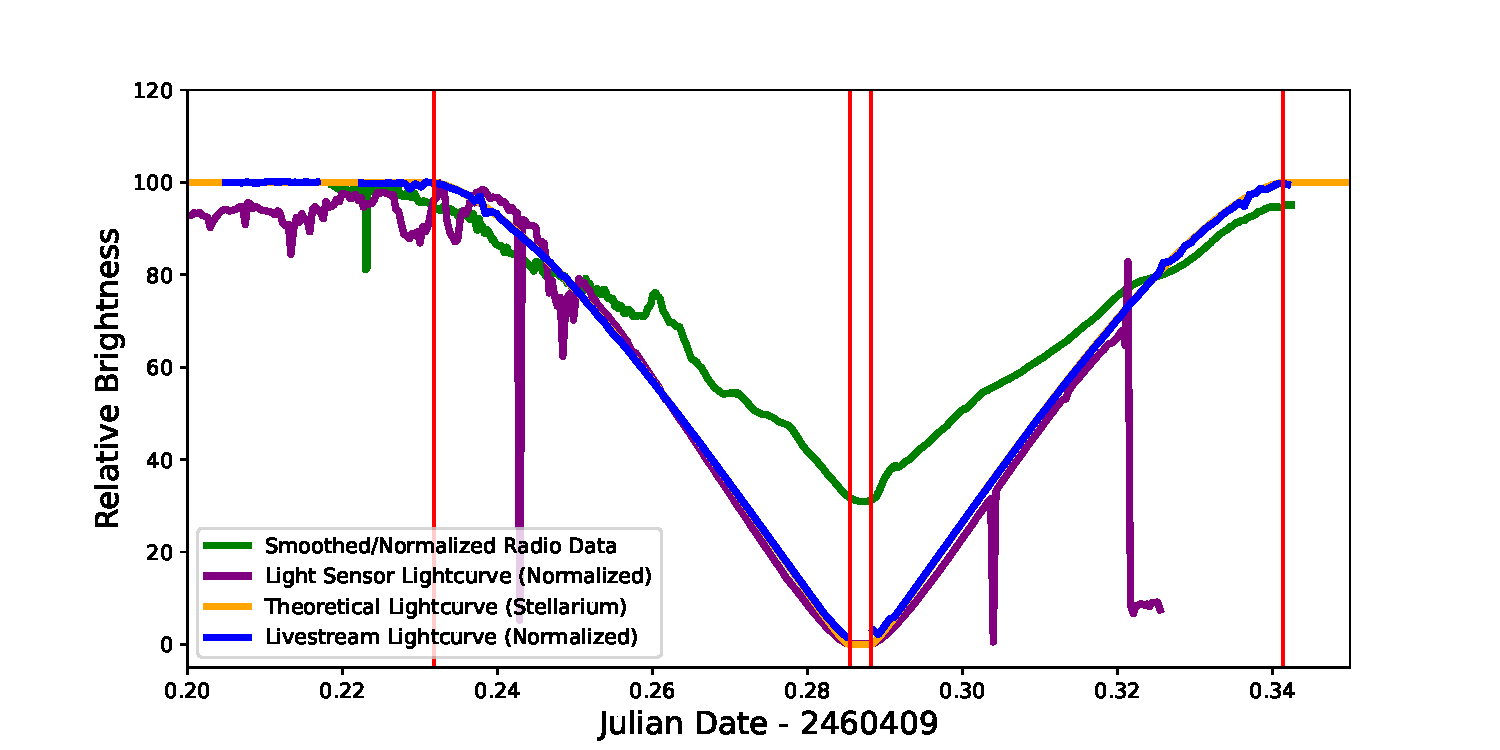
\includegraphics[width=0.9\textwidth]{figures/LightcurveComparison.pdf}
    \caption{\label{fig:LightcurveComparison} A comparison of the smoothed/normalized radio lightcurve, the normalized optical lightcurve generated from the livestream, the lightcurve generated from the light sensor, and a theoretical lightcurve generated from the software \texttt{Stellarium}. Vertical lines show first through fourth contact. \protectThe drop in the smoothed/normalized radio brightness due to the gust of wind is visible just after JD 2460409.22
.}
\end{figure}

%\begin{figure}
%  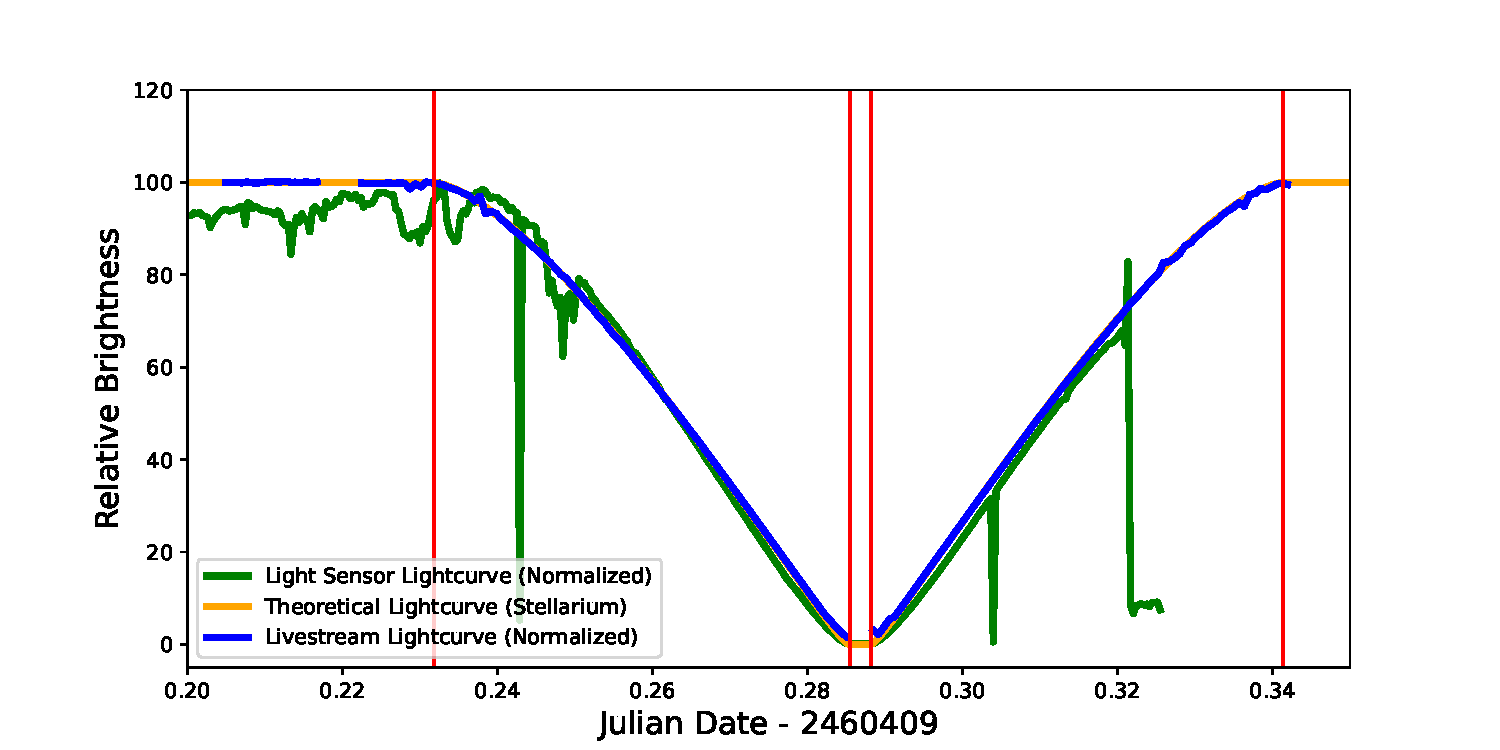
\includegraphics[width=\textwidth]{figures/OpticalComparison}
%  \caption{\label{fig:OpticalLightcurveComparison} A comparison of the livestream, light sensor, and \texttt{Stellarium} lightcurves.}
%\end{figure}


\subsection{\label{sec:optical}The Optical Lightcurve}

To better understand the features of our radio data, we need an optical lightcurve for comparison.
Ideally, the optical lightcurve would be observed from the same location as our radio telescope in order for us to compare contact times, the depth of the eclipse, and the shape of the lightcurve.
Fortunately, Dr. Scott Austin used the UCA observatory across the street from our location to livestream the eclipse using a solar filter-equipped camera mounted to the observatory telescope.
Another experiment near our location, led by Dr. Todd Abel and UCA Student Shane Ayotte, used a Vernier Light Sensor (LS-BTA) pointed straight up at the sky to measure overall sky brightness.
\paragraph{The Livestream Lightcurve}
The livestream of the solar eclipse was captured by Dr. Scott Austin using a Sony Alpha 6400 camera with a Sony FE 24mm-240mm f/3.5-6.3 lens and NiSi Solar Filter Pro Nan UV/IR Cut ND 100000 72mm filter.
This solar filter was removed during totality, marked by vertical lines at 2460409.2849 JD and 2460409.2884 JD.
This setup was attached to a Meade-14 LX200R on a Paramount MX+ equatorial mount to track the sun across the sky.
To transform the livestream into a lightcurve, we needed to extract the percentage of the sun's disk visible in the video frames as the eclipse progressed.
We accomplished this by first grayscaling the image of the eclipse and then using Otsu thresholding \cite{otsu_1979} to only count pixels above a certain value.
This sucessfully counted the bright sun pixels while ignoring the background noise.
To get the time for each data point, we took an image of the in-video clock at the same time we counted the pixels of the eclipse and used computer vision to recognise the characters in the clock, giving us the time at which the frame was pixel-counted.
The number of pixels of the solar disk over time can then be normalized to a relative brightness.
\paragraph{The Light Sensor Lightcurve}
The light sensor used to collect data during the solar eclipse was the Vernier Light Sensor (LS-BTA) pointed at the sky.
Dr. Todd Abel and Shane Ayotte provided the light sensor data, which we normalized to relative brightness.
Because the light sensor data had timestamps included, we used it to confirm the timing accuracy of our other lightcurves.

Figure \ref{fig:LightcurveComparison} shows the observed lightcurves and a theoretical lightcurve generated from the software \texttt{Stellarium}\cite{zotti_simulated_2020}, where we observed that all three optical lightcurves had a very similar shape with heavy overlap between the theoretical and livestream lightcurves.
This implies that our optical lightcurves are accurate and can be used to compare with our radio lightcurve to determine the size of the sun's radio emission.
